\subsubsection{Problem 2}
The transfer function for the travel controller in \cref{eq:P2_P} can be written as
\begin{equation}
    \frac{\td{\lambda}(s)}{\td{\lambda}_c(s)} = \frac{\rho}{s + \rho}, 
    \label{eq:P2_p_trasfer}
\end{equation}
where $\rho$ is a constant. Assuming that the pitch angle is controlled perfectly, this can be shown by rewriting \cref{eq:P1_linearised_equation_of_motion_lambda_ddot} so that
\begin{align}
    \tilde{p} &= \frac{\tdd{\lambda}}{K_3} \label{eq:P2_p_to_lambda}.
\end{align}
Inserting this into \cref{eq:P2_P} then yields
\begin{align*}
    \tdd{\lambda} &= K_3 K_{lp} (\td{\lambda}_c - \td{\lambda}),
\end{align*}
which in the laplace domain is
\begin{align*}
    s\td{\lambda} &= K_3 K_{lp} (\td{\lambda}_c - \td{\lambda}).
\end{align*}
Finally, by rearranging the terms, the transfer function becomes 
\begin{align}
    h(s) = \frac{\td{\lambda}}{\td{\lambda}_c} = \frac{K_3 K_{lp}}{s + K_3 K_{lp}},
\end{align}
which when letting $\rho = K_3 K_{lp}$ is the same as \cref{eq:P2_p_trasfer}.

To find a proper value for $K_{lp}$ one can look at the poles for both the pitch and travel controller. Because travel is dependant on pitch, pitch control should be faster than travel. From the perspective of pole placement, this means that the magnitude of the pitch poles should be greater than the travel poles.
After some trial and error, $K_{lp} = -1.15$ was found to produce a rapid response without any considerable overshoot, as can be seen in figure \cref{fig:P2p2_K_lp}. From the pole plot in figure \cref{fig:P2p2_poles} we can see that the pitch controller is much faster.
\begin{figure}[!!ht!!!!!!!!tb!!]
    \begin{minipage}{0.5\textwidth}
    	\centering
		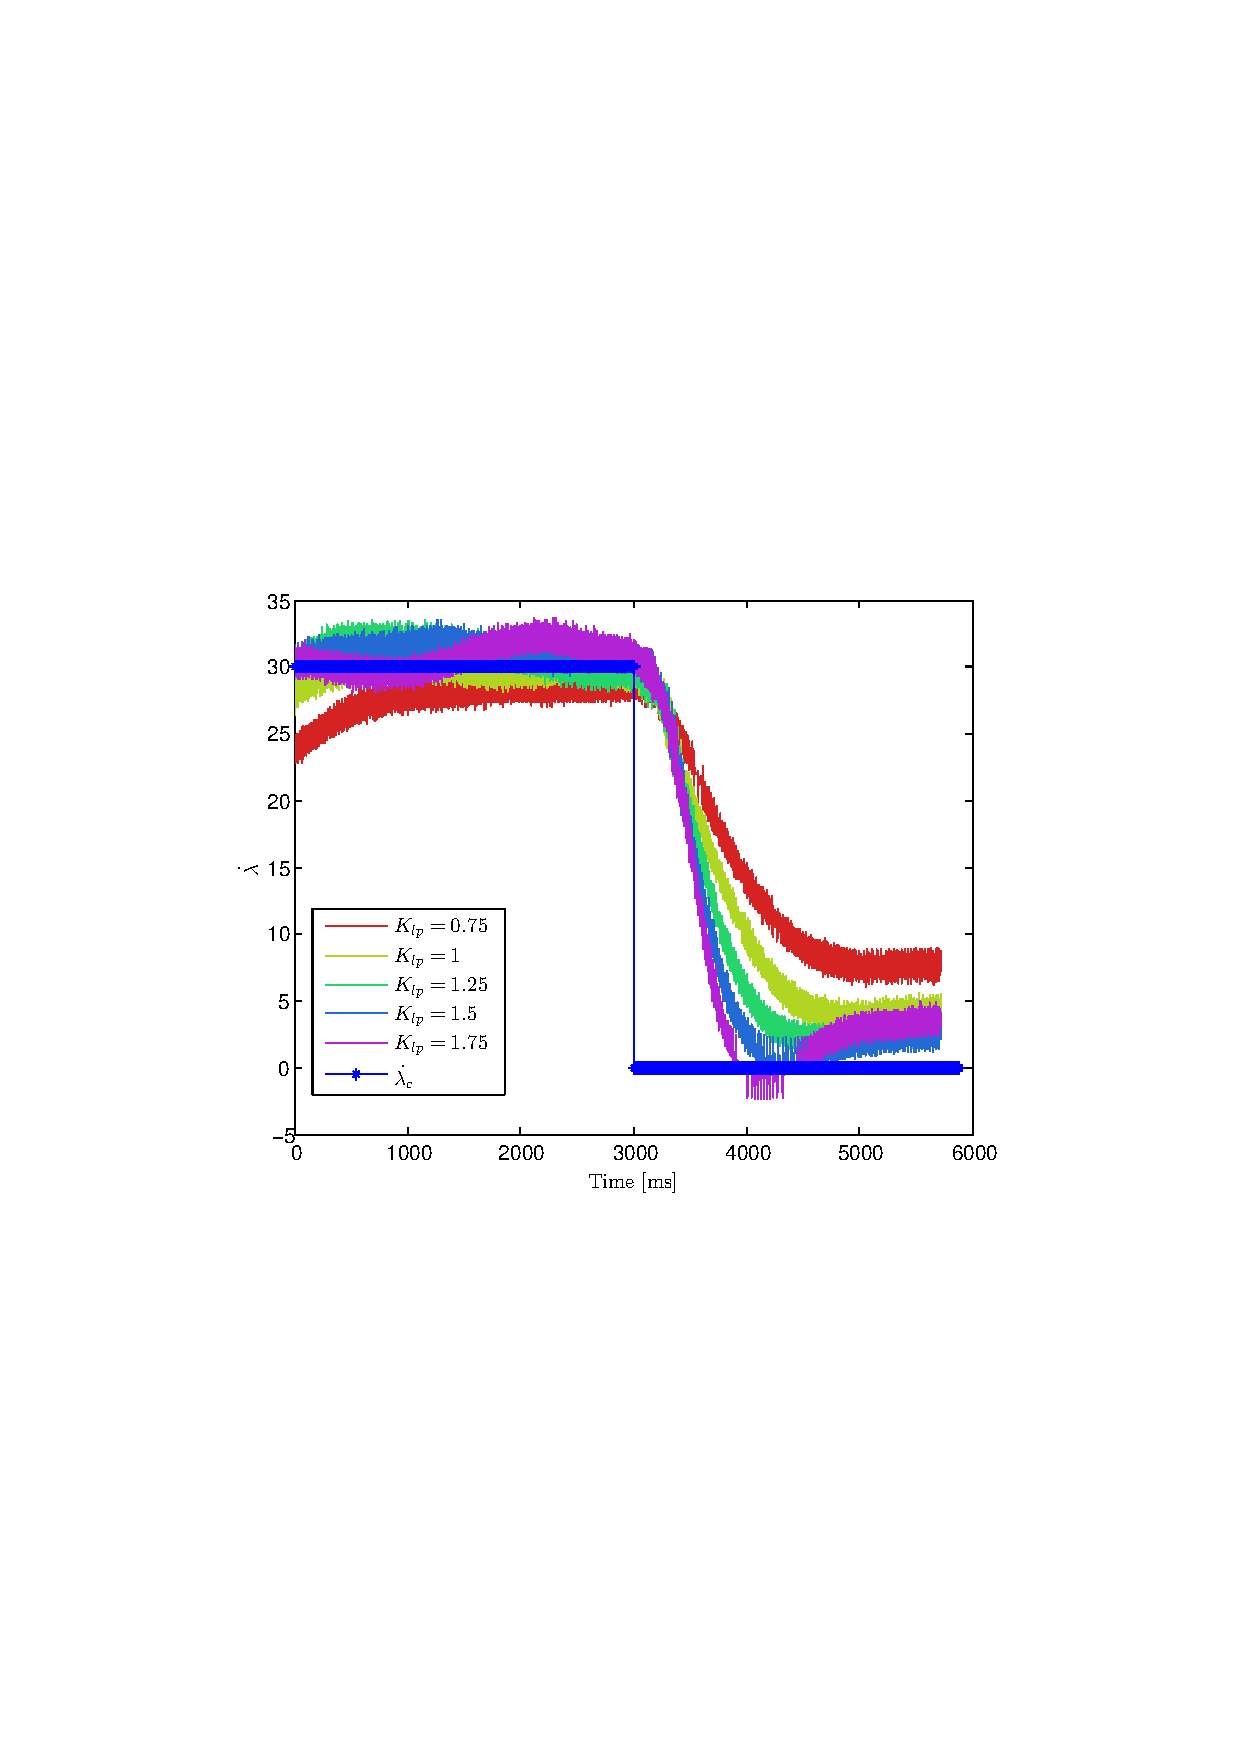
\includegraphics[width=1\textwidth,trim={4cm 9cm 4cm 9cm},clip]{figures/P2p2_Klp.pdf}
    	\caption{Travel response with P control}
	\end{minipage}
	\begin{minipage}{0.5\textwidth}
    	\centering
		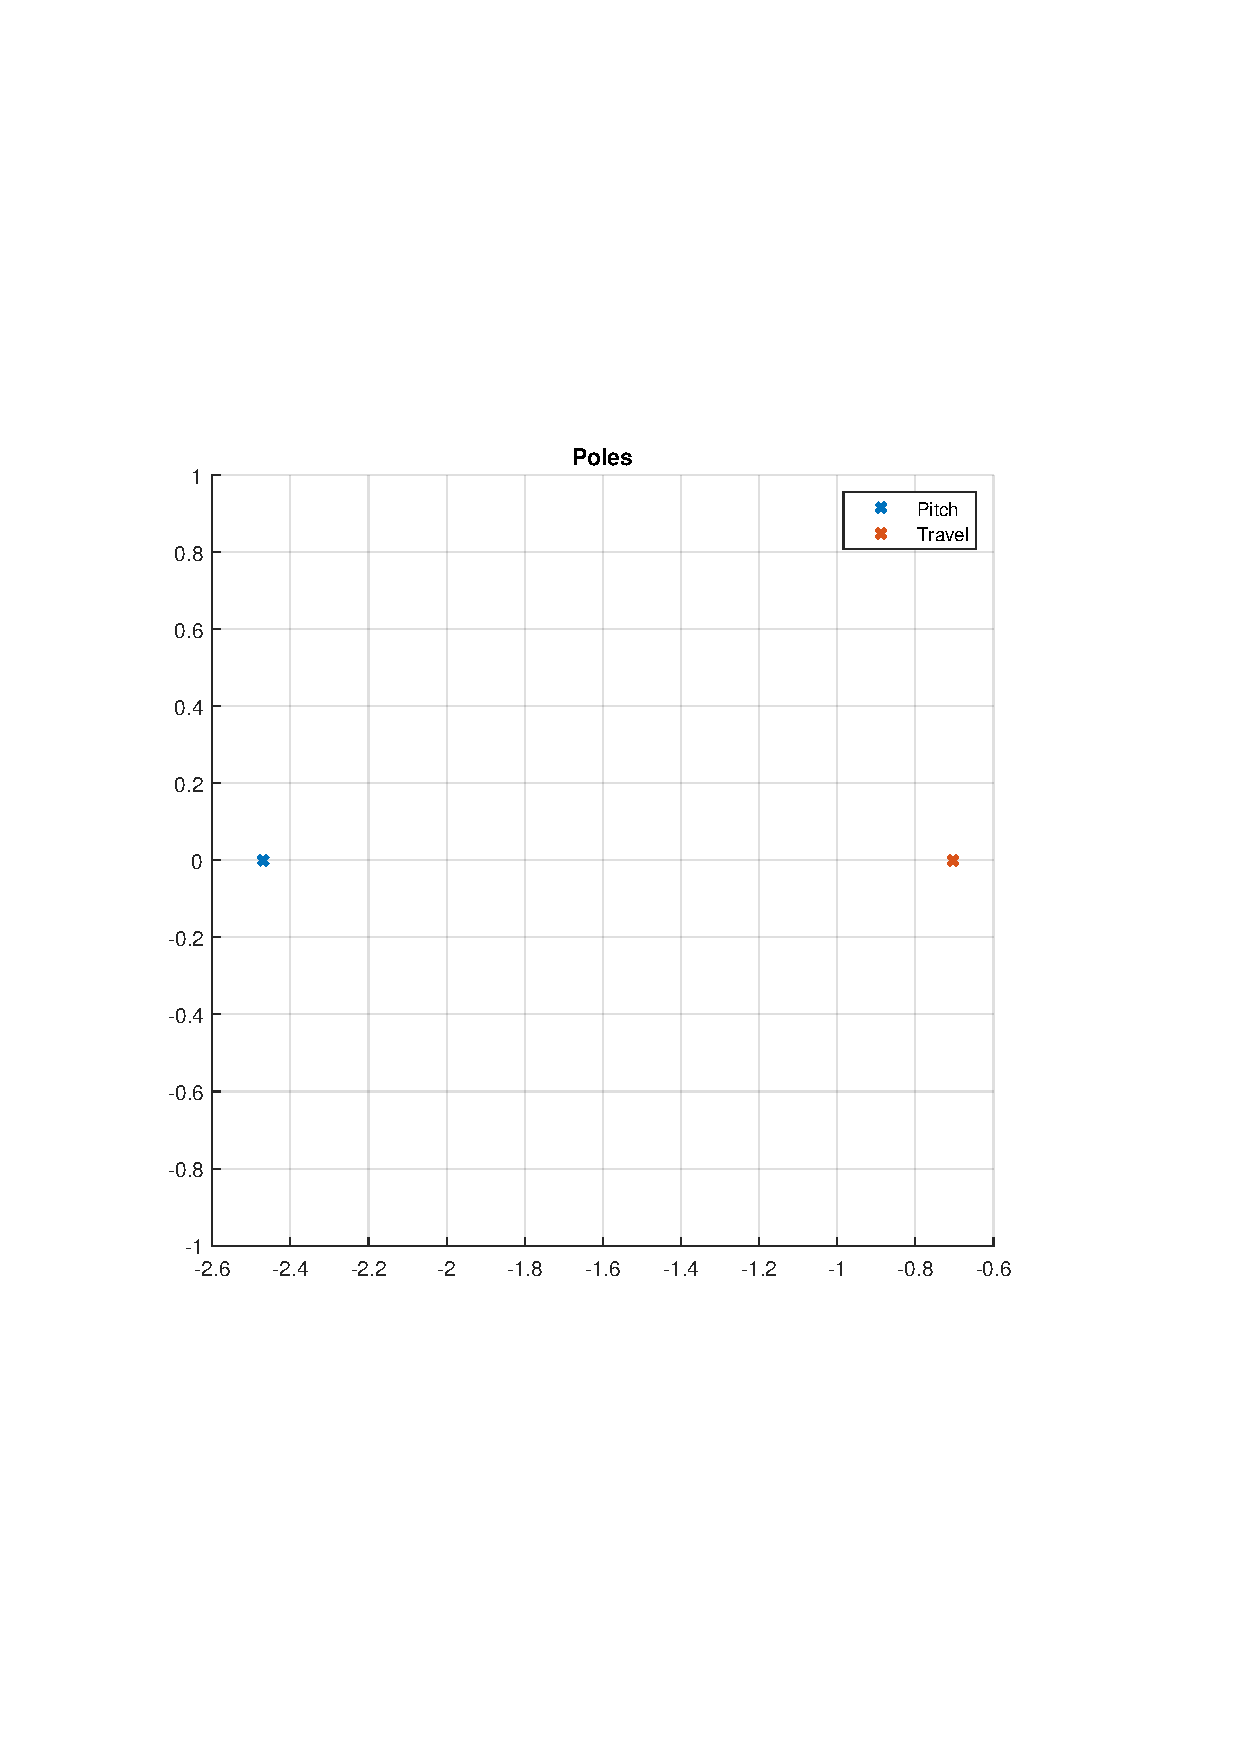
\includegraphics[width=1\textwidth,trim={2cm 7cm 3cm 6cm},clip]{figures/Travel_controller.pdf}
    	\caption{Travel and pitch controller poles}
	\end{minipage}
\label{fig:P2p2_poles}
\end{figure}
\clearpage
\begin{figure}[!!ht!!!!!!!!tb!!]
    	\centering
		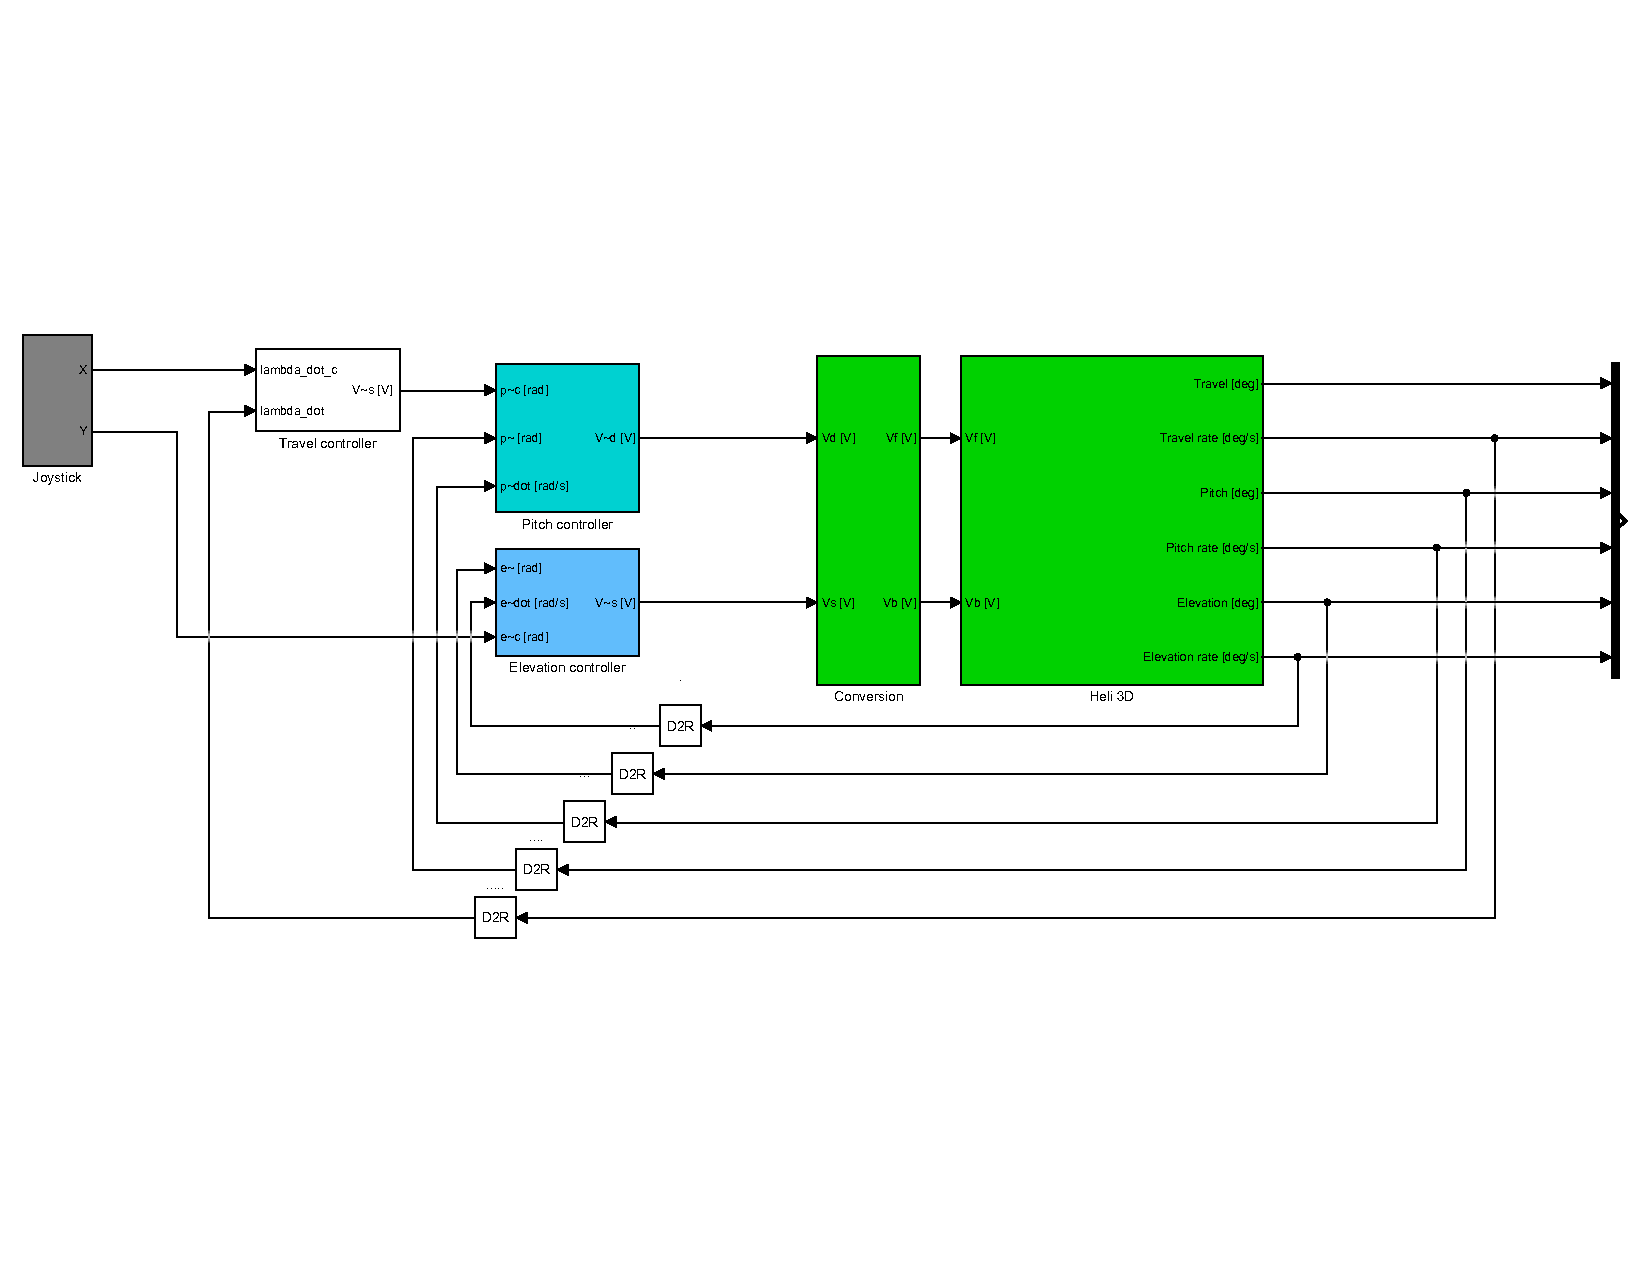
\includegraphics[width=1.1\textwidth,trim={0cm 3cm 0cm 5cm},clip]{figures/simulink/P2p2.pdf}
    	\caption{Simulink model of Part 2 problem 2}
\label{fig:P2p2_system}
\end{figure}
\begin{figure}[!!ht!!!!!!!!tb!!]
	\centering
		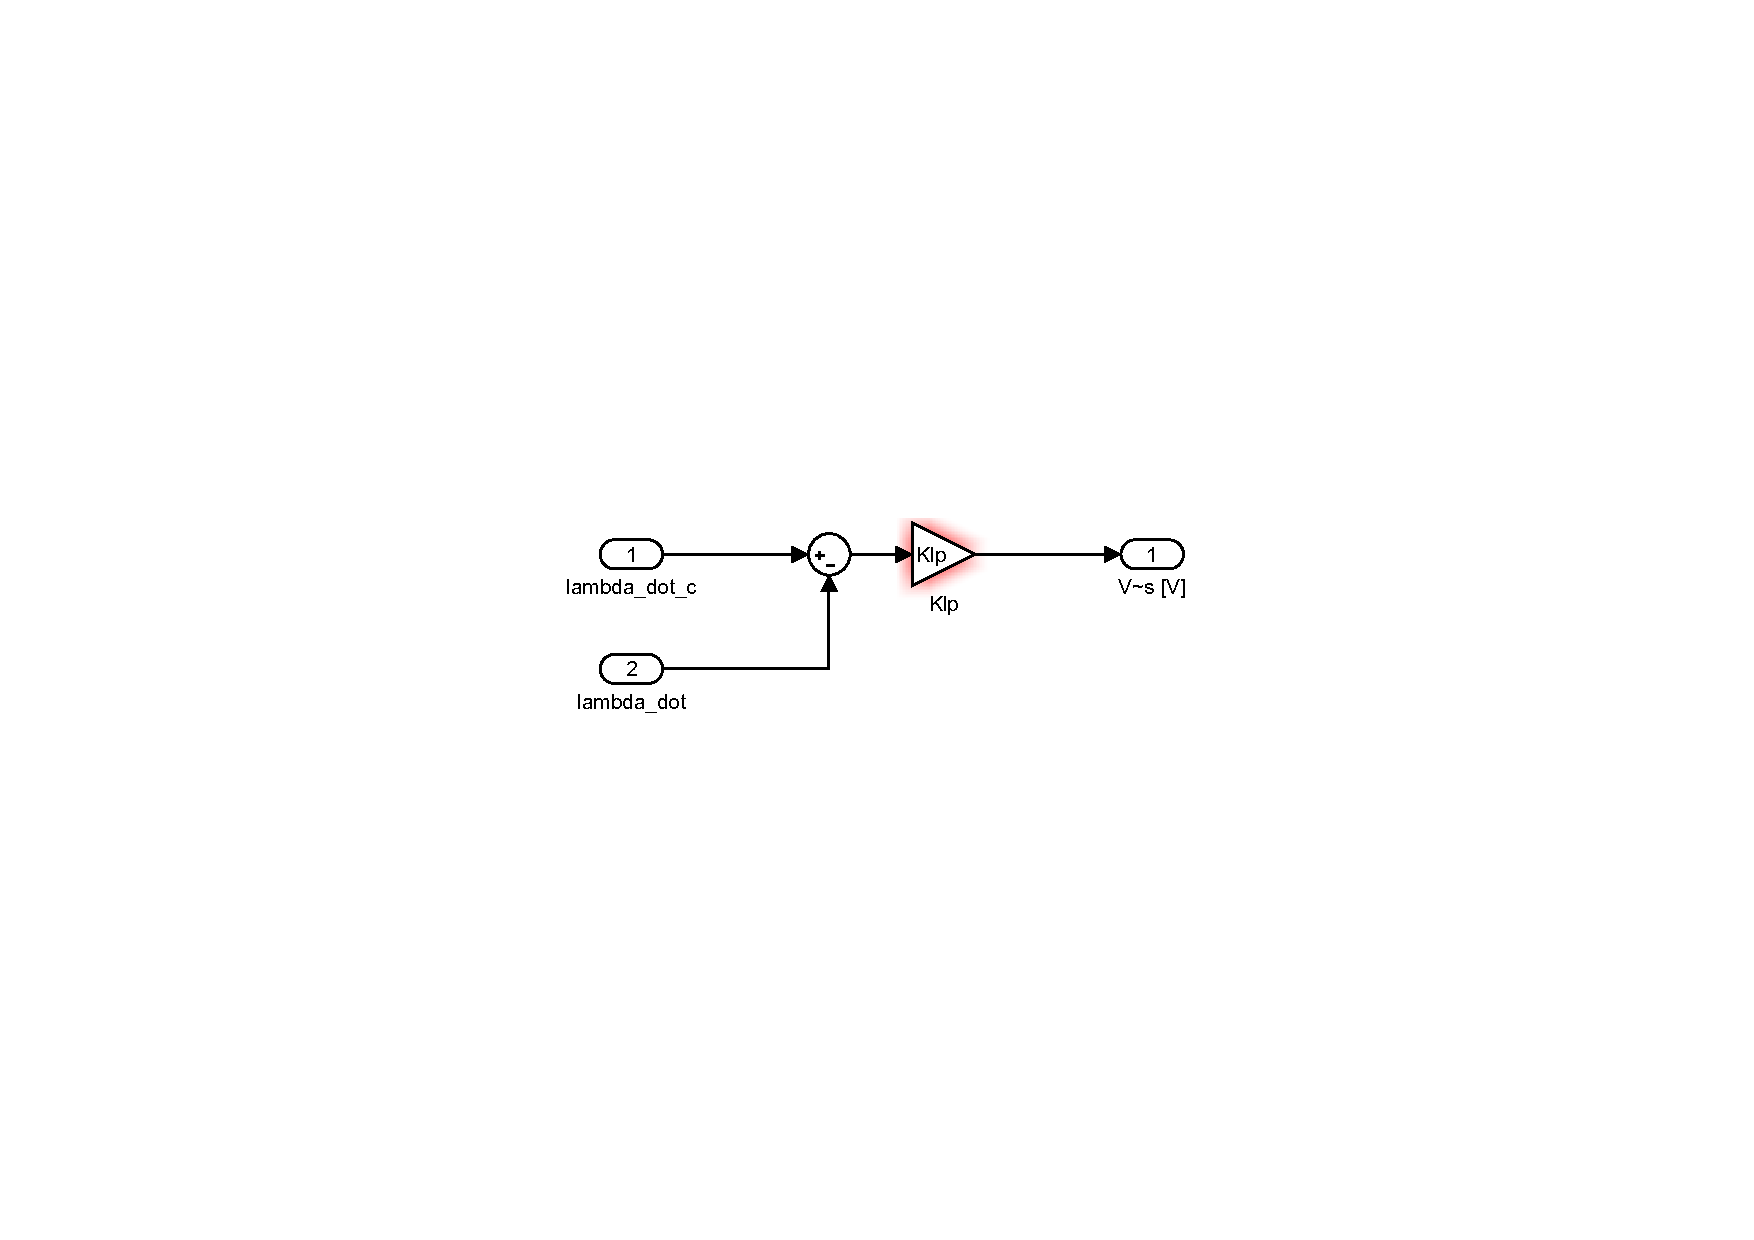
\includegraphics[scale=1.1, trim={9.2cm 8cm 0cm 4cm},clip]{figures/simulink/P_controller.pdf}
	\caption{Inside the Travel controller}
\label{fig:P2p2_controller}
\end{figure}
\clearpage